%\chapter*{Введение}
%\addcontentsline{toc}{chapter}{Введение}

\newpage
\begin{center}
\textbf{\large ГЛАВА 1 \\ Методы изучения мягкой материи на уровне отдельных частиц}
\end{center}
\refstepcounter{chapter}


% \section*{}
\addcontentsline{toc}{chapter}{ГЛАВА 1. Методы изучения мягкой материи на уровне отдельных частиц}


\section{Типы межчастичных взаимодействий}\label{C1_1}

 Взаимодействие частиц в различных системах описывается посредством потенциалов взаимодействия, основным свойством которых является отталкивание частиц на малом расстоянии и притяжение на большом. Он определяет поведение отдельных частиц и термодинамику системы в целом.
 
 К межмолекулярным взаимодействиям относятся взаимодействия между молекулами и/или атомами, не приводящие к образованию ковалентных химических связей.

Межмолекулярные взаимодействия имеют электростатическую природу. На больших расстояниях преобладают силы притяжения, которые могут иметь ориентационную, поляризационную и дисперсионную природу.

По дальности притяжения частиц частиц, взаимодействия делятся на короткодействующие и дальнодействующие. Для достаточно больших расстояний $r$ абсолютное значение потенциала двух тел ограничено $r^{-\alpha}$. Если положительная степень $\alpha$ больше, чем размерность пространства d, в которое встроена система, $\alpha>d$, система является короткодействующей, иначе, если $\alpha \leq d$, дальнодействующей.

К дальнодействующим взаимодействиям относят электростатические взаимодействия между ионами, металлическую связь и силы Ван-дер-Ваальса. 

Сильное и слабое взаимодействия являются короткодействующими. Их интенсивность быстро убывает при увеличении расстояния между частицами.  Электромагнитное и гравитационное взаимодействия являются дальнодействующими. Такие взаимодействия медленно убывают при увеличении расстояния между частицами и не имеют конечного радиуса действия.

Для изучения влияния потенциала взаимодействия на свойства веществ, в современной физике применяются так называемые модельные системы. В них частицы выступают в роли атомов и молекул, а возможность регулирования взаимодействий в таких системах, позволяет изучить процессы, происходящие в реальных веществах.

Среди модельных систем наибольший интерес представляют коллоидные системы во внешнем электрическом поле,в котором в отличии, например, от пылевой плазмы, возможно реализовать не только отталкивающие взаимодействия \cite{gel3}, но так же и притяжение, посредством наложения внешнего вращающегося электрического поля, которое вызывает диполь-дипольное притяжение \cite{gel6}.

Рассмотрим процессы, происходящие в коллоидных системах подробнее. 

Как правило, из-за разного материала частиц и сольвента возникает притяжение Ван-дер-Ваальса \cite{Yur31, Yur53}:
\begin{equation}
\varphi_{\mathrm{vdW}}(r)=-\frac{A_{\mathrm{H}}}{12}\left(\frac{\sigma^{2}}{r^{2}-\sigma^{2}}+\frac{\sigma^{2}}{r^{2}}+2 \ln \frac{r^{2}-\sigma^{2}}{r^{2}}\right)
\end{equation}
где постоянная Хамакера $A_{\mathrm{H}} \propto\left(\frac{\varepsilon_{\mathrm{r}}-1}{\varepsilon_{\mathrm{r}}+1}\right)^{2}$ зависит от относительной диэлектрической проницаемости $\varepsilon_{\mathrm{r}}=\varepsilon_{\mathrm{P}} / \varepsilon_{\mathrm{S}}$. 

Предотвращению коагуляции, в коллоидной системе способствуют силы отталкивания, которые обусловлены зарядовой или стерической стабилизацией.

Зарядовая стабилизация возникает благодаря взаимному отталкиванию заряженных частиц, в результате накопленного на их поверхности отрицательного заряда, который возникает при диссоциации поверхности и адсорбции ионов. 
В рамках линеаризованной теории Пуассона--Больцмана, взаимодействие Дерягина--Ландау--Фервея--Овербека имеет вид \cite{Yur54}:
\begin{equation}
\varphi_{Y}(r)=\left\{\begin{array}{ll}
\infty & r<\sigma, \\
\epsilon_{\mathrm{Y}} \frac{e^{-\kappa(r-\sigma)}}{r / \sigma} & r \geq \sigma,
\end{array}\right.
\end{equation}

где $\kappa=\sqrt{4 \pi \lambda_{\mathrm{B}} n_{\mathrm{ion}}} \equiv \lambda_{\mathrm{D}}^{-1}$ - обратная дебаевская длина экранирования, выраженная через плотность малых ионов $n_{ion}$ и длину Бьеррума $\lambda_{\mathrm{B}}=e^{2} / \varepsilon_{\mathrm{w}} k_{\mathrm{B}} T$. Контактный потенциал записывается как 

\begin{equation}
\epsilon_{\mathrm{Y}}=\frac{Z^{2}}{(1+\kappa \sigma / 2)^{2}} \frac{\lambda_{\mathrm{B}}}{\sigma} k_{\mathrm{B}} T,
\end{equation}
где $Z \equiv Q / e$ зарядовое число коллоида.

Результирующее взаимодействие представляет собой сумму притягивающих и отталкивающих сил:
\begin{equation}
\varphi(r)=\varphi_{Y}(r)+\varphi_{\mathrm{vdW}}(r).
\end{equation}
Вклады данных слагаемых соизмеримы на малом расстоянии между не сильно заряженными частицами.

С ростом заряда частиц, теория Пуассона--Больцмана становится неприменимой вблизи поверхности частицы, однако на дальних расстояния по прежнему имеет форму Юкавы, и при ренормированном зарядом может хорошо описывать потенциал вдали от поверхности \cite{Yur55}. Эффективный насыщенный заряд выражается следующим уравнением \cite{Yur56}
\begin{equation}
Z_{\mathrm{eff}}^{\mathrm{sat}}=(2+\kappa \sigma) \sigma / \lambda_{\mathrm{B}}
\end{equation}
Используя линеаризованную теорию Пуассона - Больцмана с установленным эффективным зарядом, можно объяснить большинство экспериментальных наблюдений \cite{Yur57, Yur58, Yur59}. Это делает теорию Дерягина-Ландау-Фервея-Овербека (ДЛФО) одним из наиболее успешных подходов при описании межчастичных взаимодействий \cite{Yur49, Yur60, Yur61}. 

Помимо зарядовой стабилизации существует так называемая стерическая стабилизация. Она заключается в добавлении в сольвент полимерных молекул, которые оседают на частицах. При сближении, эти полимерные цепи взаимодействуют друг с другом, не давая частицам сблизиться сильнее. 

Часть потенциала взаимодействия, которая соответствует стерической стабилизации, выглядит следующим образом \cite{Yur31}
\begin{equation}
\begin{array}{l}
\varphi_{\text {steric }}(r)=\frac{\pi \sigma}{2} \int_{r-\sigma}^{\infty} d h F(h) \\
\\
F(r)=\frac{\alpha k_{\mathrm{B}} T}{s^{3}}\left[\left(\frac{2 L}{r}\right)^{9 / 4}-\left(\frac{r}{2 L}\right)^{3 / 4}\right], \quad r<2 L
\end{array}
\label{eqStericStabl}
\end{equation}
где $L$ - толщина полимерного слоя, $\alpha$ - численный множитель, определяемый для конкретных полимеров
особенностями взаимодействия между молекулярными цепочками, $s$ - среднее расстояние между привитыми полимерами на поверхности.

В случае наличия этих взаимодействий, суммарный потенциал частиц выражается следующей формулой:

\begin{equation}
\varphi(r)=\varphi_{Y}(r)+\varphi_{\mathrm{vdW}}(r)+\varphi_{\mathrm{steric}}(r).
\end{equation}

Помимо сила Ван-дур-Вальса, на притяжение между частицами также может повлиять внешнее электрическое поле \cite{gel6}.

Однако данное взаимодействие не является анизотропным, из-за чего частицы выстраиваются вдоль линии поля. Для того, чтобы этого избежать, внешнее поле меняет направление с периодом меньшим, чем период релаксации ионной оболочки вокруг коллоидной частицы. Это позволяет сделать притяжение частиц в системе изотропным.

\begin{figure}[h]
\begin{center}
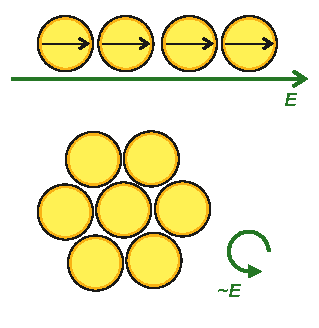
\includegraphics[width=0.5\textwidth]{Управляемое взаимодействие направленное поле}
\caption{Частицы расположенные сверху, находятся в стационарном внешнем электрическом поле, что делает их взаимодействие анизотропным. Частицы расположенные снизу, находятся в вращающимся  внешнем электрическом поле, что делает их взаимодействие изотропным.}
\label{risPolar}
\end{center}
\end{figure}

При наложении внешнего поля на коллоидную систему, частица поляризуется и потенциал взаимодействия выглядит следующим образом \cite{gel7}:
\begin{equation}
\varphi(\mathbf{r})=-\mathbf{E}_{0} \cdot \mathbf{r}+\sum_{\alpha} \int_{\Gamma^{\alpha}} \mathrm{d} S \sigma^{\alpha}\left(\mathbf{r}_{k}\right) G\left(\mathbf{r}, \mathbf{r}_{k}^{\alpha}\right),
\end{equation}
где $r_{k}^{\alpha} \in \Gamma^\alpha, \Gamma^\alpha$ - поверхность $\alpha$-ой частицы, $G\left(\mathbf{r}, \mathbf{r}_{k}^{\alpha}\right)$ - функция Грина в уравнении Лапласа, и суммирование проводится по всем частицам.

Данное уравнение решается численными методами, и при усреднении по углу позволяет довольно точно описывать коллоидные частицы во внешних электрических полях.

Это позволяет использовать коллоидные системы как модельные, для изучения свойств мягкой материи на уровне отдельных частиц. 

\section{Модельные потенциалы взаимодействий}

Для изучения влияния микроскопических свойств системы на макроскопические, используется так называемый метод \textbf{молекулярной динамики (МД)}, который заключается в численном моделировании системы, состоящей из достаточно большого количества частиц, по статистике которых можно судить о макроскопических свойствах. 

Данные моделирования заключаются в численном решение уравнений Ньютона для каждой отдельной частицы. Одним из преимуществ такого подхода является возможность создания систем с совершенно любыми потенциалами взаимодействия между частицами. Он позволяет моделировать эффекты разрушения, пластичность, температурное изменение свойств материала, фазовые переходы.

Одним из наиболее популярных модельных потенциалов взаимодействия частиц в таких системах, является потенциал Леннарда - Джонса:
\begin{equation}
U\left(R_{i j}\right)=\varepsilon\left[\left(\frac{R_{0}}{R_{i j}}\right)^{12}-2\left(\frac{R_{0}}{R_{i j}}\right)^{6}\right]=4 \varepsilon\left[\left(\frac{\sigma}{R_{i j}}\right)^{12}-\left(\frac{\sigma}{R_{i j}}\right)^{6}\right], 
\label{eqFullLJ}
\end{equation}
где $\varepsilon$ и $R_0$ - глубина потенциальной ямы и равновесное расстояние между частицами; $R_0 = 2^{1/6}\sigma$.

В то время как зависимость $R^{-6}$ получена теоретически и обусловлена силами Ван-дер-Ваальса, зависимость $R^{-12}$ выбрана из соображений удобства.

\begin{figure}[h]
\begin{center}
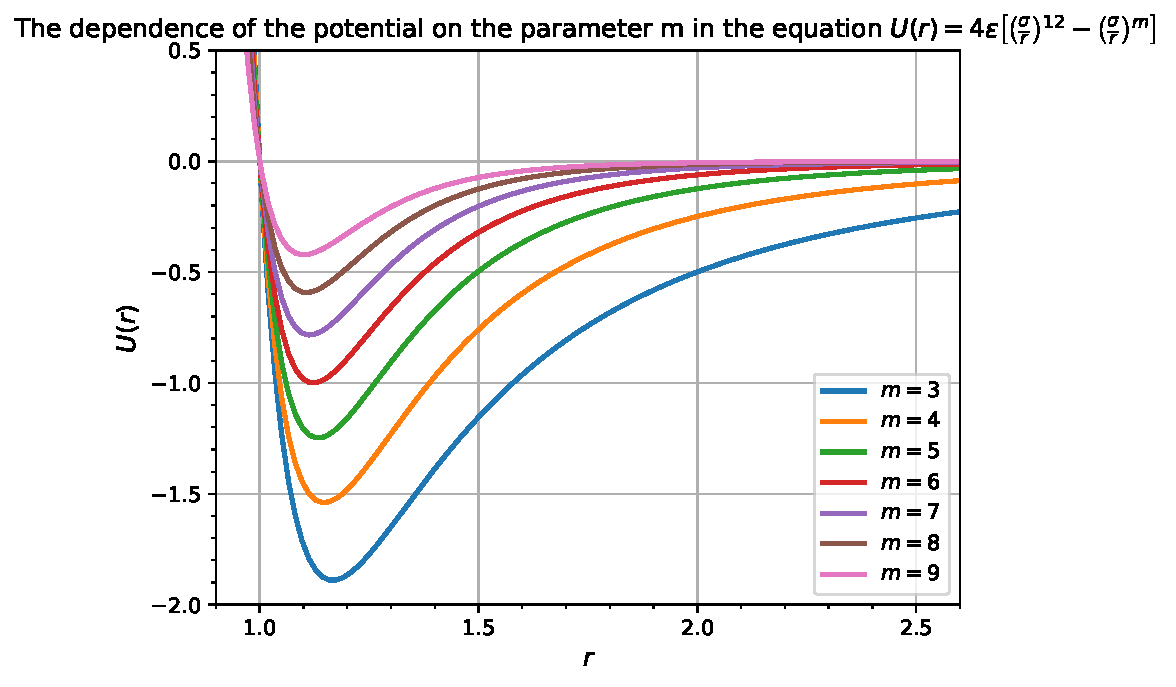
\includegraphics[width=\textwidth]{LJ}
\caption{Демонстрация обобщенного потенциала Леннарда--Джонса с различными степенями слагаемого, отвечающего за притяжение. $m = 6$ соответствует стандартному потенциалу Леннарда--Джонса.}
\label{risLJvar}
\end{center}
\end{figure}

Потенциал Леннарда--Джонса является простейшим из всех видов потенциалов у которого потенциальная энергия зависит от модуля расстояния между частицами. Несмотря на сильно ограниченные возможности в количестве макроскопических параметров, из-за наличия всего двух варьируемых параметров, потенциал весьма точно описывает свойства ряда веществ (прежде всего, кристаллических инертных газов), а также достаточно точно описывает силы взаимодействия \\ Ван--дер--Ваальса, играющие важную роль в твердых телах. К достоинству потенциала Леннарда--Джонса относится так же его вычислительная простота, не требующая вычисления иррациональных и трансцендентных функций.

Во многие модельных системах, такие как коллоидные суспензии и пылевые плазмы, парные взаимодействия на коротких расстояниях в основном описываются отталкиванием Юкавы \cite{phase59}.

Система точечных частиц в 2D геометрии, взаимодействует через попарно отталкивающий потенциал вида:
\begin{equation}
\varphi(r)=\frac{\varepsilon \lambda}{r} \exp \left(-\frac{r}{\lambda}\right)
\end{equation}

где $\varepsilon, \lambda$ - энергетические и экранирующие масштабы длин взаимодействия. Для заряженных частиц, погруженных в плазмоподобную экранирующую среду, энергетическая шкала равна:
\begin{equation}
\varepsilon=Q^{2} / 4 \pi \epsilon_{0} \lambda
\end{equation}

где $Q$ - заряд, $\epsilon_{0}$ - диэлектрическая проницаемость пространства.

Свойства систем Юкавы определяются двумя параметрами: параметром связи и параметром отбора. Первый определяется так:
\begin{equation}
\text{Г}=Q^{2} / 4 \pi \epsilon_{0} a k_{\mathrm{B}} T
\end{equation}

где $k_b$ - постоянная Больцмана, T - температура, $a=(\pi n)^{-1 / 2}$ - радиус Вигнера-Зейтца, где n - концентрация частиц на единицу объема.

Второй параметр равен:
\begin{equation}\kappa=a / \lambda\end{equation}

Заметим, что параметр связи - отношение потенциальной энергии взаимодействия двух соседних частиц к их кинетической энергии. Обычно говорят, что система находится в сильно связанном состоянии, когда это соотношение велико \cite{phase59}.

Различные физические величины в данных моделированниях удобно выражать через константы моделирования. В случае Леннарда-Джонса это  $\sigma, \varepsilon, m$, где $m$ - масса частиц, $\sigma$ - расстояние, на котором энергия взаимодействия становится равным нулю, $\varepsilon$ - глубина потенциальной ямы.

Метод молекулярной динамики, в данной работе, позволяет выяснить влияние дальнодействия притяжения на термодинамические свойства системы и параметры переноса.

\section{Цели и задачи бакалаврской работы}

\textbf{Цель работы} --
установить связь между дальнодействием притяжения в двумерной системе частиц, взаимодействующих посредством обобщенного потенциала Леннарда-Джонса, c фазовой диаграммой, и параметрами переноса.

\textbf{Задачи работы:}
\begin{enumerate}
\item Разработка программного комплекса для расчета явлений переноса в $2D$ системах.
\item Разработка методов определения термодинамических свойств системы по распределениям плотностей. 
\item Усовершенствование метода распознавание фаз и построения фазовых диаграмм.
\item Применение разработанных методов на различных потенциалах взаимодействия.
\item Применение наработок для изучения влияния потенциала взаимодействия на различные термодинамические параметры.
\end{enumerate}
